\documentclass{anstrans}
%%%%%%%%%%%%%%%%%%%%%%%%%%%%%%%%%%%
\title{Modeling Reactor Neutronic Transient using Gaussian Processes}
\author{Rabab Elzohery}

\institute{
Department of Mechanical \& Nuclear Engineering, Kansas State University, Manhattan, KS 66506
}


%%%% packages and definitions (optional)
\usepackage{graphicx} % allows inclusion of graphics
\usepackage{booktabs} % nice rules (thick lines) for tables
\usepackage{microtype} % improves typography for PDF
\usepackage{multirow}
\usepackage{float}
\usepackage{siunitx}
\usepackage{amsmath,bm}

\newcommand{\SN}{S$_N$}
\renewcommand{\vec}[1]{\bm{#1}} %vector is bold italic
\newcommand{\vd}{\bm{\cdot}} % slightly bold vector dot
\newcommand{\grad}{\vec{\nabla}} % gradient
\newcommand{\ud}{\mathop{}\!\mathrm{d}} % upright derivative symbol

\begin{document}
%%%%%%%%%%%%%%%%%%%%%%%%%%%%%%%%%%%%%%%%%%%%%%%%%%%%%%%%%%%%%%%%%%%%%%%%%%%%%%%%

\section{Abstract}
Simplified models that approximate the outputs of high fidelity models are needed to overcome the 
problem of the high computational cost associated with such models.\\
Moreover, these models suffer from what so called the curse of dimensionality. Hence, reduction techniques 
are often applied in these approximate models.\\
In this study, a linear model has been developed to approximate the response of a numerical experiment. The experiment represents a neutronic transient in a reactor core in which the response has both spatial and temporal dependence. 
A reduction has been done in the spatial domain and the flux is decomposed into spatial modes each weighted by a temporal coefficient, while Gaussian processes (GP) was used to build a linear model to approximates these coefficients.\\
With proper choice of the correlation function, results show that the model was able to recover the response  with an average error of order $10^{-11}$ .

\section{Introduction}
High-fidelity models are of large use in different research areas in nuclear engineering. However, because they perform a very detailed simulation of the underlying physics, they are computationally demanding.
Some of the real-world problems such as design optimization and uncertainty quantification require repetitive evaluation of the model, which makes these applications computationally prohibitive.
Hence, simplified models, a.k.a surrogate models that are computationally cheaper and reasonably accurate are often sought to carry out such calculations.\\
Moreover, most of these simulations employ some numerical schemes which solve the problem in a discrete manner in space/time. For better accuracy, most of the problems are solved over a very fine mesh resulting in high dimensional input/output space.
However, there always exist a spatial/temporal correlation between the model inputs and also, the responses of interest. 
Such correlation can be exploited to build these approximate models in terms of lower number of dimensions which are called reduced order models (ROM). 
This idea of reducing the input/output dimensionality is closely related to that of the variables transformation.

Reduced order models can be classified as intrusive and non-intrusive methods. Intrusive method include projection methods which requires access to the source code and modifying the underlining equations, non-intrusive method are purely data-driven.\\
In this study, a linear reduced order model has been developed to a approximate the output of a numerical experiment. This experiment represents a class of problems of interest in the nuclear field, namely, reactor transients. 
The Final goal is to use this model to propagate input uncertainties and compute the uncertainties in some responses of interest.
The response of interest is the neutron population (i.e neutron flux) in the reactor which exhibits a non-linear behavior in both space and time as a result of control rod movements inside the reactor core. The spatial averaged flux is shown in fig.\ref{fig:neutron flux}.\\
\begin{figure}
    \centering
    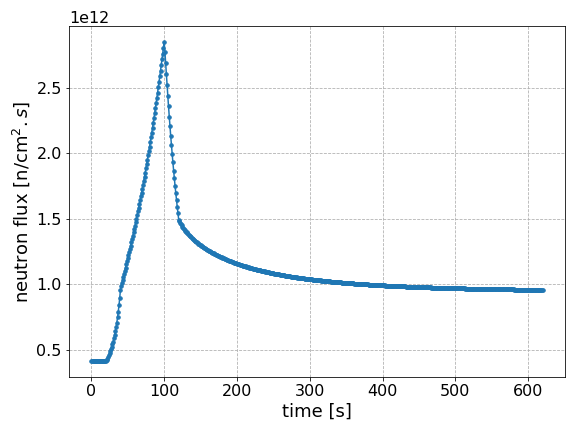
\includegraphics[scale=0.4]{./figs/ave_flux.png}
    \caption{Neutron Flux}
    \label{fig:neutron flux}
\end{figure}
In a previous work, different reduced-order models were developed for the same problem, of which a model based on the POD-Galerkin projection gave a very promising results. 
However, the method required modification in the governing equations.
Here, a close idea is adopted but with using a Gaussian process model which is completely data-driven . 
Detailed description of the model is given in the next section.

\section{Methods}
The method proposed here involves two steps. First, a reduction in the output space or transformation of the responses is performed, so that they can be explained in terms of some spatial basis.
Then a linear model is built for the expansion coefficients of these basis as a function of time. 
\subsection{Reduction}
One of the most common ways to explore the potential of data for reduction is the proper orthogonal decomposition (POD), also known as principal component analysis (PCA).
The basic idea of the PCA is to transform the correlated input/output variables so that they can be explained in terms of uncorrelated lower number of dimensions, which is performed by diagonalizing the data correlation matrix.\\
Mathematically, this can be done using the singular value decomposition (SVD). Consider a data matrix $\textbf{Y} \in \mathcal{R}^{m\times n}$,  where $m$ is the number of spatial dimensions and $n$ is the number of data snapshots at different times. The SVD of $\textbf{Y}$ is computed as follows, 
\begin{equation}
 \textbf{Y} =\textbf{U}\boldsymbol{\Sigma}\textbf{V}^T;
\end{equation}

where $\textbf{U}$ and $\textbf{V}$ are orthogonal matrices containing the left and right singular vectors respectively, $\boldsymbol{\Sigma}$ is a diagonal matrix containing the singular values, 
which can be interpreted as the variance of the data along the corresponding left singular vector, i.e, the columns of $\textbf{U}$. 
Thus, by inspecting the singular values, a reduction can be made by keeping only the first $r$ singular values and the corresponding $r$ columns of $\textbf{U}$ and $\textbf{V}$.
Figure \ref{fig:svd} shows the normalized singular values, which strongly suggests the potential of data for reduction, 
\begin{figure}[!h]
	\centering
	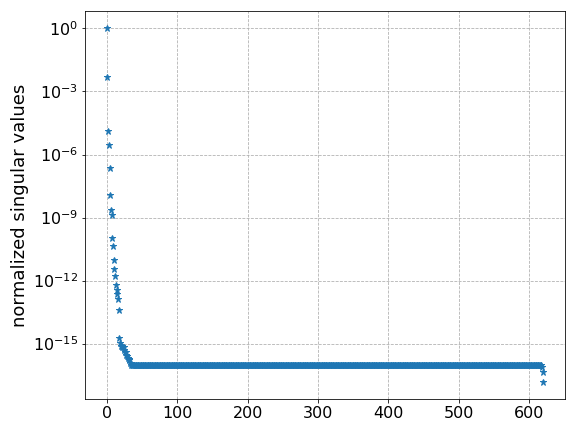
\includegraphics[scale=0.4]{./figs/singular_values.png}
	\caption{Normalized singular values}
	\label{fig:svd}
\end{figure}

\subsection{Transformation}

A widely used method to approximate a high dimensional spatio-temporal data, in engineering applications, is the POD-Garlekin projection, in which the quantity of interest can be approximated as; 

\begin{equation}
\textbf{y} = \bar{\textbf{y}}(x) + \sum_{i=1}^r \textbf{u}_i a_i(t)
\label{pod-galerkin}
\end{equation}
where $\bar{\textbf{y}}$ is the mean of response, and the other term represents the fluctuation of the data around the mean, which is a linear combination of the dominant POD modes or the principal components, assembled in $\textbf{U}_r$, each weighted by a temporal coefficient.
Now, the problem remains in finding the coefficients $\textbf{a}(t)$.
In POD-Galerkin projection, this is achieved by projecting the physical system, which is represented by a system of coupled PDEs, onto the space of $\textbf{U}_r$, thus reducing it from $n$ to $r$ equations.
However, this requires knowledge of these equation and modifying the source code.
Hence, in this work, a statistical linear model is proposed to approximate these coefficients. For the sake of brevity, only the first four coefficients are shown in figure \ref{fig:coeffs}.\\
\begin{figure}[!h]
	\centering
	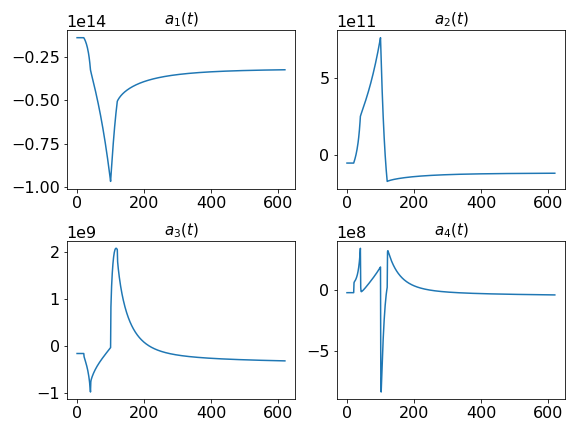
\includegraphics[scale=0.4]{./figs/temp_coeff.png}
	\caption{The temporal coefficients a(t)}
	\label{fig:coeffs}
\end{figure}
Once these coefficients are computed, the responses can be transformed back to its original space, i.e $\textbf{Y} = \textbf{U}^T \textbf{a}$.
\subsection{The linear Model}
The temporal coefficients $\textbf{a}(t)$ can be approximated by a general linear model with the following form,  
    \begin{equation}
    \textbf{a(t)} \sim \mathcal{N} ({\boldsymbol{\beta}}, \textbf{K}+ \sigma^2I)
    \end{equation}
Where, $\textbf{K}$ is a general covariance function, and $\sigma^2$ is the variance of the residual.

Another way to look at the model, is that it is the projection of equation \ref{pod-galerkin} onto the space of $\textbf{U}_r$, but with adding a random effect or an extra assumption of the errors correlations.
Such models are known as Guassian processes \cite{rasmussen2003gaussian} and they involve the choice of a trend function which represents the mean of the predicted value, and also a correlation function. 
Different options can be used for the correlation function. The most commonly used one is the exponential square, also known as the radial basis function (RBF), and it has the following form,
 \begin{equation}
  K(x_i, x_j) =  exp(-\frac{(x_i - x_j)^2}{2l^2})
\end{equation}
where $l > 0$ is hyper-parameter. The model parameters can be estimated by a Bayesian technique, or by maximizing the likelihood function.

\section{Results}
The method presented in the previous section was used to recover the time dependent flux $\textbf{Y} \in \mathcal{R}^{700\times 621}$. The scikit-learn library in python\cite{scikit-learn} was used to develop the model, since it supports different correlation functions.
Based on the singular values shown in figure \ref{fig:svd}, only 20 principal components or POD modes were kept which is a meaningful reduction. Thus, a Gaussian process model with 20 outputs was built. Note that without this transformation, the output space size would be 700.\\
A fitted model with a constant trend function is developed. Different correlation functions are tried to   select a model with a correlation function that gives the best error in the recovered data. \\
The mean and the variance of the predicted flux were computed following algorithm 2-1 in \cite{rasmussen2003gaussian}. The hyperparameters of the covariance function are optimized during fitting by maximizing the log-marginal-likelihood (LML).
The correlation functions that were used are the radial based function(RBF), Marten, Rational quadratic and Exp-Sine-Squared functions.
For details on the structure of each function, the reader might refer to \cite{rasmussen2003gaussian}. Also, a covariance function with constant variance is used.\\
Using the predicted flux, the core power was computed. Figure \ref{gp_kernels} shows the absolute residual in the core power with different covariance functions.
Also, as part of the outputs, the variance at each data point is computed, which gives the $95\%$ confidence interval. However, it was very small that it can not be shown in the figure.
\begin{figure}[ht!]
	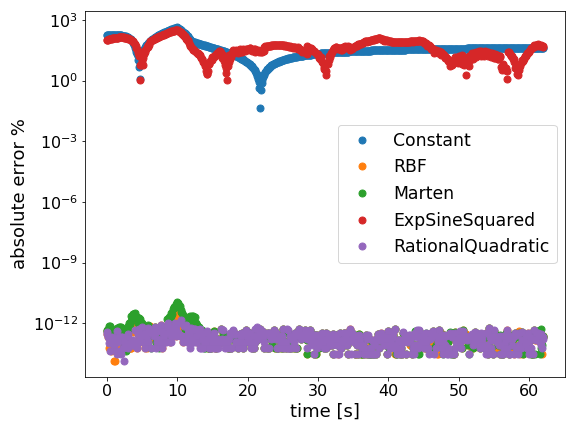
\includegraphics[scale=0.4]{./figs/gp_kernels.png}
	\caption{Absolute error in the predicted flux}
	\label{gp_kernels}
\end{figure}


\section{Discussion}
The results in the previous section show that the models with the RBF, rational quadratic and Martin correlation functions are able to recover the data within a very good accuracy. 
These three kernels have connection with each other and they are all characterized by length scale parameter ($l$) which can be interpreted as the range over which each point has affect on the other points.
While these three correlation give similar error, the RBF function might be a better choice since it has less hyperparameters which makes performing the optimization calculations faster.
However, the constant and the Exp-Sine-Squared models did not perform well, which is expected since the constant kernel assumes that the correlation between the data points are the same, which is not the case as shown in figure \ref{fig:coeffs}. 
Furthermore, the Exp-sind-squared functions are best fit for periodic functions which is also not the case here.

As compared to the previously developed surrogate models for the same problem, this surrogate gives better error. So it might be useful to investigate the method more on different case studies for the same class of problems. 
Another case study for more complicated problem is given in  along with a tutorial of this work and materials required to reproduce these results \cite{RababGit}.

As mentioned before, the final goal of this surrogate is to be used to propagate uncertainties through. Hence, a future work will involve using this model to compute the distribution of the response of interest given a known distribution of some physical input parameters, in which case Bayesian technique could be more suitable, related work has been done in \cite{assessing} .

 
%%%%%%%%%%%%%%%%%%%%%%%%%%%%%%%%%%%%%%%%%%%%%%%%%%%%%%%%%%%%%%%%%%%%%%%%%%%%%%%%
\bibliographystyle{ans}
\bibliography{bibliography}
\end{document}

